\documentclass[11pt]{article}

\usepackage[margin=0.85in]{geometry}
\usepackage[T1]{fontenc}
\usepackage[utf8]{inputenc}
\usepackage{lmodern}
\usepackage{microtype}
\usepackage{amsmath, amssymb, mathtools}
\usepackage{booktabs}
\usepackage{array}
\usepackage{longtable}
\usepackage{enumitem}
\usepackage{xcolor}
\usepackage{hyperref}
\usepackage{pdflscape}
\usepackage{tikz}
\usetikzlibrary{arrows.meta, positioning, fit, calc, backgrounds, shapes.geometric}

\hypersetup{
    colorlinks=true,
    linkcolor=blue!60!black,
    urlcolor=blue!60!black,
    citecolor=blue!60!black
}

\definecolor{boxblue}{RGB}{220,235,252}
\definecolor{boxgreen}{RGB}{223,242,228}
\definecolor{boxorange}{RGB}{252,236,214}
\definecolor{boxred}{RGB}{248,224,224}
\definecolor{boxgray}{RGB}{238,238,238}
\definecolor{boxpurple}{RGB}{232,225,246}

\tikzset{
  mybox/.style={
    draw,
    rounded corners=2.5pt,
    thick,
    align=center,
    minimum height=9mm,
    inner sep=2.5pt,
    font=\small
  },
  data/.style={mybox, fill=boxgreen},
  op/.style={mybox, fill=boxblue},
  train/.style={mybox, fill=boxorange},
  note/.style={mybox, fill=boxgray},
  future/.style={mybox, fill=boxpurple},
  critical/.style={mybox, fill=boxred},
  arr/.style={-Latex, thick},
  arrthin/.style={-Latex, semithick}
}

\title{Repository Plan for \texttt{mini-llm-lab}}
\author{Project design document}
\date{\today}

\begin{document}
\maketitle

\section{Purpose of the repository}

This repository is meant to be a learning platform for building a small modern
\textbf{large language model (LLM)} from the ground up while keeping the mathematics,
the matrices, and the numerical flow visible.

The central idea is:

\begin{quote}
Every important part of the model should be inspectable as explicit matrices,
explicit tensor operations, and explicit backward derivatives.
\end{quote}

The project is therefore \emph{not} primarily about obtaining the strongest model
possible. Instead, it is about understanding:

\begin{itemize}[leftmargin=1.5em]
    \item how text becomes tokens,
    \item how tokens become vectors,
    \item how \textbf{Transformer} blocks propagate information,
    \item how \textbf{attention} works,
    \item how residual connections work,
    \item how the next-token prediction loss is formed,
    \item how gradients move backward through the model, and
    \item how optimization updates the matrices.
\end{itemize}

\section{Main design philosophy}

The repository follows the following rules.

\subsection*{Rule 1: explicit numerical objects}
All trainable weights should appear as visible matrices, usually through a small
\texttt{Parameter} class with:
\[
\texttt{data}, \qquad \texttt{grad}.
\]

\subsection*{Rule 2: explicit forward pass}
Each module should compute its forward operation with explicit tensor contractions,
for example:
\[
Q = XW_Q,\qquad K = XW_K,\qquad V = XW_V,
\]
rather than hiding the operation behind a high-level neural-network framework layer.

\subsection*{Rule 3: explicit backward pass}
Each module should also contain its own hand-derived backward pass.
For example, if
\[
Y = XW,
\]
then the backward formulas are:
\[
\frac{\partial L}{\partial W} = X^\top \frac{\partial L}{\partial Y},
\qquad
\frac{\partial L}{\partial X} = \frac{\partial L}{\partial Y}W^\top.
\]

\subsection*{Rule 4: CPU first, GPU second}
The same code should run with:
\begin{itemize}[leftmargin=1.5em]
    \item \textbf{NumPy} for a clear \textbf{central processing unit (CPU)} reference implementation,
    \item \textbf{CuPy} for \textbf{graphics processing unit (GPU)} acceleration.
\end{itemize}

\subsection*{Rule 5: verify before scaling}
Every operator should be tested numerically before being integrated into a larger model.
In practice this means:
\begin{itemize}[leftmargin=1.5em]
    \item directional derivative checks,
    \item finite-difference tests,
    \item shape checks,
    \item causality checks for attention,
    \item and small overfitting experiments.
\end{itemize}

\section{Acronyms and terms}

\begin{longtable}{p{0.18\linewidth} p{0.77\linewidth}}
\toprule
\textbf{Term} & \textbf{Meaning} \\
\midrule
LLM & Large language model. A neural network trained to predict the next token in text. \\
CPU & Central processing unit. The ordinary processor of the computer. \\
GPU & Graphics processing unit. A highly parallel processor used for accelerated tensor operations. \\
BPE & Byte-pair encoding. A tokenizer method that merges frequent token pairs to build a vocabulary. \\
LM & Language model. In this repository, usually a decoder-only next-token prediction model. \\
GQA & Grouped-query attention. A variant of attention where several query heads share the same key and value heads. \\
RoPE & Rotary positional embedding, more precisely a rotary positional transformation applied to query and key vectors. \\
RMSNorm & Root-mean-square normalization. A normalization layer using the root mean square of the input vector. \\
FFN & Feed-forward network. In this project, the position-wise non-attention block inside a Transformer block. \\
SwiGLU & Swish Gated Linear Unit. A feed-forward structure using a SiLU (sigmoid linear unit) gate. \\
MoE & Mixture of experts. A sparse feed-forward structure in which a router activates only some experts for each token. \\
KV cache & Key-value cache. Saved keys and values used during autoregressive generation to avoid recomputing the whole prefix. \\
CE loss & Cross-entropy loss. The loss used for next-token prediction. \\
AdamW & An optimization method based on Adam with decoupled weight decay. \\
SFT & Supervised fine-tuning. A later-stage training step used to teach instruction-following behavior. \\
\bottomrule
\end{longtable}

\section{Repository structure}

The repository is planned to evolve toward the following structure:

\begin{verbatim}
mini_llm_lab/
|-- mini_llm/
|   |-- backend.py
|   |-- config.py
|   |-- init.py
|   |-- parameter.py
|   |-- ops/
|   |   |-- linear.py
|   |   |-- embedding.py
|   |   |-- rmsnorm.py
|   |   |-- rope.py
|   |   |-- attention.py
|   |   |-- swiglu.py
|   |   `-- loss.py
|   |-- optim/
|   |   |-- adamw.py
|   |   |-- grad_clip.py
|   |   `-- schedule.py
|   |-- diagnostics/
|   |   `-- gradcheck.py
|   |-- blocks/
|   |   |-- transformer_block.py
|   |   `-- moe.py
|   |-- model/
|   |   |-- decoder_lm.py
|   |   `-- inference.py
|   `-- data/
|       |-- tokenizer.py
|       |-- preprocess.py
|       `-- dataloader.py
|-- tests/
|-- examples/
`-- docs/
\end{verbatim}

\section{Planned milestones}

\subsection*{Milestone 1: numerical primitives (already started)}
Implemented or being implemented:
\begin{itemize}[leftmargin=1.5em]
    \item backend selection (NumPy / CuPy),
    \item parameter objects,
    \item initialization,
    \item linear layers,
    \item embedding lookup,
    \item RMSNorm,
    \item RoPE,
    \item grouped-query causal attention,
    \item SwiGLU,
    \item cross-entropy loss,
    \item gradient clipping,
    \item AdamW,
    \item numerical derivative checks.
\end{itemize}

\subsection*{Milestone 2: dense Transformer block}
Build the standard dense Transformer block:
\[
X \rightarrow \text{RMSNorm} \rightarrow \text{Attention} \rightarrow +X
\rightarrow \text{RMSNorm} \rightarrow \text{SwiGLU} \rightarrow +X.
\]

\subsection*{Milestone 3: dense decoder language model}
Stack multiple Transformer blocks, tie the input embedding matrix to the output
language-model head, and train a small decoder-only language model on a tiny corpus.

\subsection*{Milestone 4: sparse feed-forward replacement}
Replace the dense feed-forward network by a \textbf{mixture of experts (MoE)} block:
\[
\text{Dense FFN} \;\longrightarrow\; \text{Router} + \text{Experts}.
\]

\subsection*{Milestone 5: data pipeline}
Build the tokenizer and dataset pipeline:
\begin{itemize}[leftmargin=1.5em]
    \item raw documents,
    \item training/validation split,
    \item tokenizer training,
    \item token packing,
    \item binary token shards.
\end{itemize}

\subsection*{Milestone 6: full training loop}
Create:
\begin{itemize}[leftmargin=1.5em]
    \item checkpoints,
    \item logging,
    \item learning-rate schedules,
    \item validation,
    \item and loss/gradient statistics.
\end{itemize}

\subsection*{Milestone 7: inference}
Add:
\begin{itemize}[leftmargin=1.5em]
    \item autoregressive decoding,
    \item sampling,
    \item key-value cache,
    \item prompt processing.
\end{itemize}

\subsection*{Milestone 8: research experiments}
Compare:
\begin{itemize}[leftmargin=1.5em]
    \item dense vs. MoE,
    \item AdamW vs. Muon,
    \item data mixtures,
    \item and routing behavior.
\end{itemize}

\section{Model overview}

The full model will be a decoder-only Transformer for next-token prediction.

\subsection{Input text and tokenization}
A raw text sequence such as
\[
\texttt{"The fluid velocity increases near the wall."}
\]
is converted to discrete token identifiers using a tokenizer such as \textbf{byte-pair encoding (BPE)}:
\[
[t_0, t_1, \dots, t_{T-1}].
\]

\subsection{Embedding}
Each token identifier is converted into a vector through an embedding matrix
\[
E \in \mathbb{R}^{V \times d_{\text{model}}},
\]
where:
\begin{itemize}[leftmargin=1.5em]
    \item \(V\) is the vocabulary size,
    \item \(d_{\text{model}}\) is the model dimension.
\end{itemize}
If \(X_0\) denotes the embedded token sequence, then
\[
X_0 \in \mathbb{R}^{B \times T \times d_{\text{model}}},
\]
where \(B\) is the batch size and \(T\) is the sequence length.

\subsection{Transformer block}
Each Transformer block contains two residual branches.

\paragraph{Attention branch.}
\[
Z_1 = \mathrm{RMSNorm}(X),
\]
\[
Q = Z_1 W_Q,\qquad K = Z_1 W_K,\qquad V = Z_1 W_V.
\]
Then RoPE is applied to \(Q\) and \(K\). Next, causal grouped-query attention is evaluated:
\[
S = \frac{QK^\top}{\sqrt{d_h}} + M,
\]
where \(M\) is the causal mask. The attention probabilities are
\[
P = \mathrm{softmax}(S),
\]
and the context is
\[
C = PV.
\]
After output projection,
\[
A = C W_O,
\]
the residual update gives:
\[
X' = X + A.
\]

\paragraph{Feed-forward branch.}
\[
Z_2 = \mathrm{RMSNorm}(X'),
\]
then the SwiGLU feed-forward network computes:
\[
G = Z_2 W_{\text{gate}},\qquad U = Z_2 W_{\text{up}},
\]
\[
H = \mathrm{SiLU}(G)\odot U,
\]
\[
F = H W_{\text{down}}.
\]
The second residual update gives:
\[
Y = X' + F.
\]

\subsection{Stacking}
If there are \(L\) layers, the sequence passes through:
\[
X_0 \rightarrow X_1 \rightarrow X_2 \rightarrow \cdots \rightarrow X_L.
\]

\subsection{Final normalization and logits}
After the last block:
\[
Z_{\text{final}} = \mathrm{RMSNorm}(X_L).
\]
The logits are then computed using the tied embedding matrix:
\[
\text{logits} = Z_{\text{final}} E^\top.
\]

\subsection{Next-token prediction}
For each position \(t\), the model predicts the next token:
\[
p(x_{t+1}\mid x_{\le t}) = \mathrm{softmax}(\text{logits}_t).
\]
Training uses the mean cross-entropy loss over all positions.

\section{Numerical conventions and initialization}

The initial implementation uses:
\begin{itemize}[leftmargin=1.5em]
    \item clipped normal initialization for most matrices,
    \item smaller standard deviation for residual-output matrices,
    \item \(\gamma = 1\) for RMSNorm gains,
    \item AdamW optimization,
    \item global gradient clipping,
    \item warmup and cosine learning-rate decay.
\end{itemize}

The main reason is not fashion; it is numerical stability and interpretability.
A transparent project is easier to debug when:
\begin{itemize}[leftmargin=1.5em]
    \item activation scales are monitored,
    \item gradient scales are monitored,
    \item the optimizer is simple and explicit,
    \item and each matrix has a clear role.
\end{itemize}

\section{How training will be validated}

Before any serious training run, the repository should verify:

\begin{enumerate}[leftmargin=1.5em]
    \item \textbf{Operator checks:} each layer passes local finite-difference checks.
    \item \textbf{Block checks:} a full Transformer block passes directional derivative checks.
    \item \textbf{Model checks:} the full dense model passes end-to-end gradient tests on a tiny example.
    \item \textbf{Memorization checks:} the model can intentionally overfit a tiny corpus.
    \item \textbf{Scaling checks:} only after the above are correct do we train on larger corpora.
\end{enumerate}

\section{Planned future MoE extension}

Later, the dense feed-forward branch will be replaced by a sparse MoE block.

The idea is:
\begin{itemize}[leftmargin=1.5em]
    \item a router computes a score for each expert,
    \item only the top-\(k\) experts are selected,
    \item the selected expert outputs are combined,
    \item and this replaces the ordinary dense feed-forward transformation.
\end{itemize}

This makes it possible to study:
\begin{itemize}[leftmargin=1.5em]
    \item sparse conditional computation,
    \item expert specialization,
    \item routing statistics,
    \item load balancing,
    \item and domain-sensitive expert behavior.
\end{itemize}

\begin{landscape}
\section*{Full model diagram}

\begin{center}
\resizebox{1.20\textheight}{!}{%
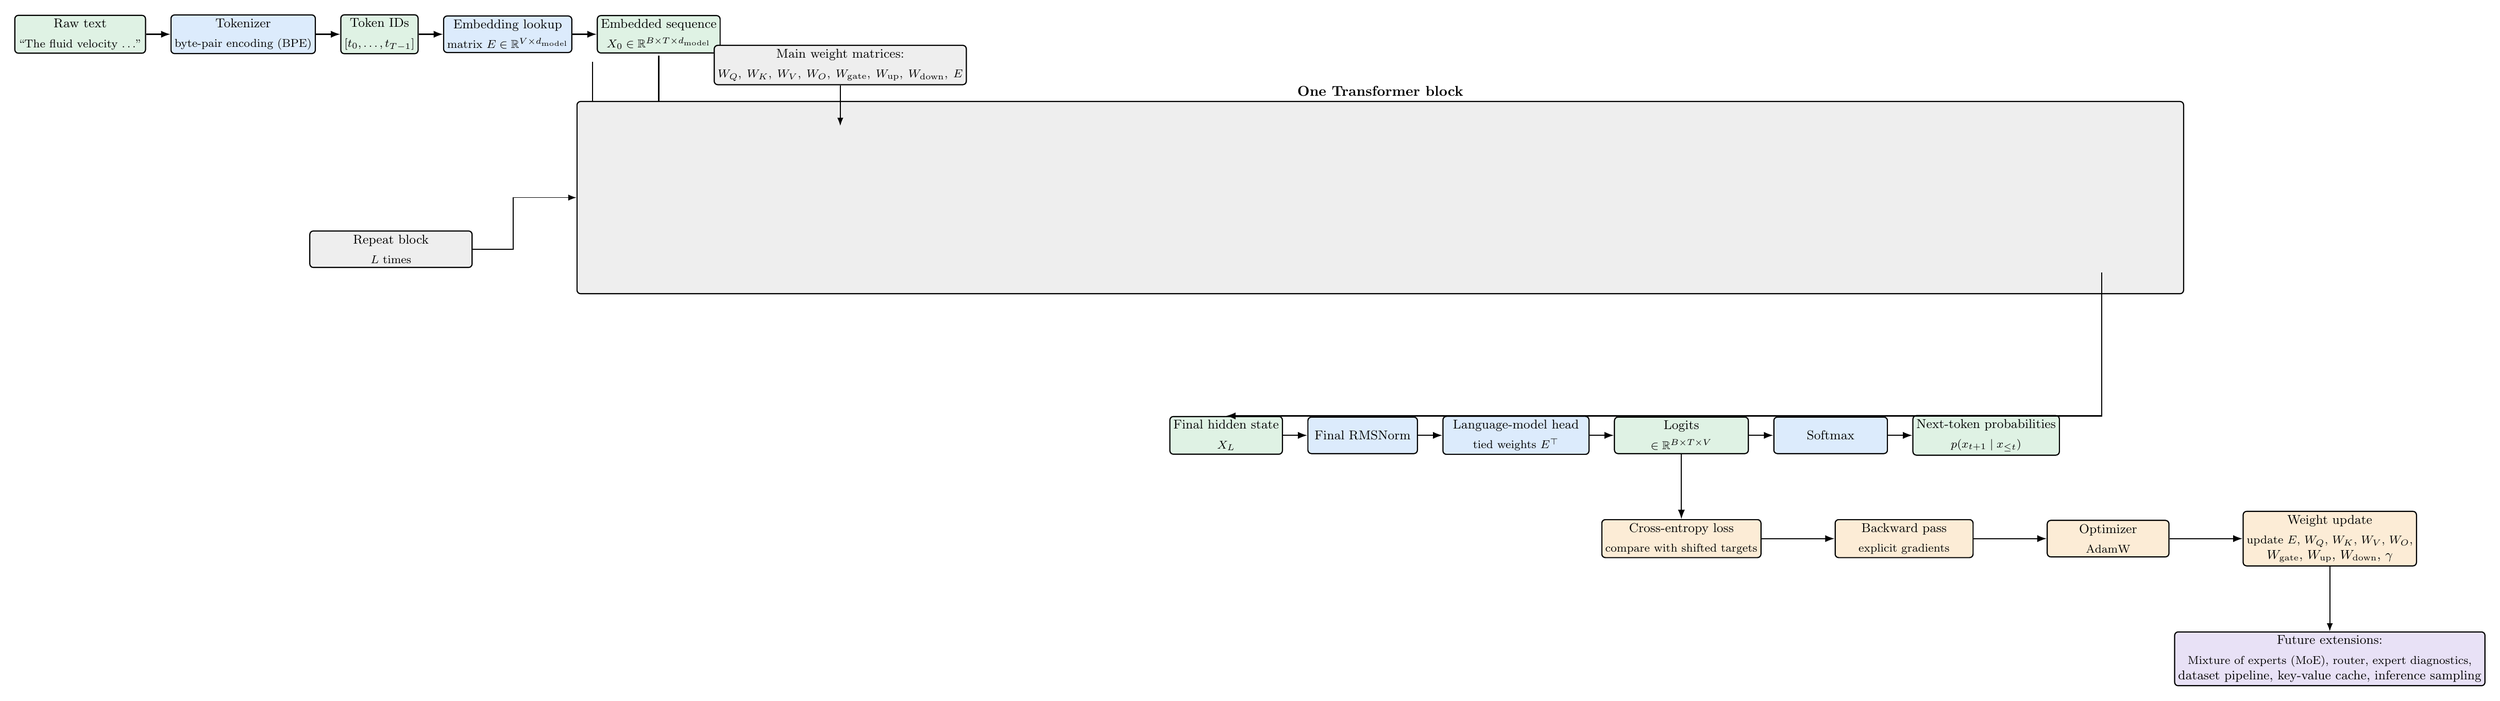
\begin{tikzpicture}[node distance=5mm and 6mm]

% Row 1
\node[data] (text) {Raw text\\[1mm]\footnotesize ``The fluid velocity $\ldots$''};
\node[op, right=of text] (tok) {Tokenizer\\[1mm]\footnotesize byte-pair encoding (BPE)};
\node[data, right=of tok] (ids) {Token IDs\\[1mm]\footnotesize $[t_0,\dots,t_{T-1}]$};
\node[op, right=of ids] (embed) {Embedding lookup\\[1mm]\footnotesize matrix $E \in \mathbb{R}^{V \times d_{\text{model}}}$};
\node[data, right=of embed] (x0) {Embedded sequence\\[1mm]\footnotesize $X_0 \in \mathbb{R}^{B \times T \times d_{\text{model}}}$};

\draw[arr] (text) -- (tok);
\draw[arr] (tok) -- (ids);
\draw[arr] (ids) -- (embed);
\draw[arr] (embed) -- (x0);

% Transformer block container
\node[op, below=18mm of x0, minimum width=28mm] (norm1) {RMSNorm\\[1mm]\footnotesize gain $\gamma_1$};
\node[op, right=of norm1, minimum width=38mm] (proj) {QKV projections\\[1mm]
\footnotesize $Q=XW_Q,\;K=XW_K,\;V=XW_V$};
\node[op, right=of proj, minimum width=25mm] (rope) {RoPE\\[1mm]\footnotesize on $Q$ and $K$};
\node[op, right=of rope, minimum width=40mm] (attn) {Causal GQA attention\\[1mm]
\footnotesize $P=\mathrm{softmax}(QK^\top/\sqrt{d_h}+M)$};
\node[op, right=of attn, minimum width=26mm] (wo) {Output projection\\[1mm]\footnotesize $A=CW_O$};
\node[critical, right=of wo, minimum width=26mm] (res1) {Residual add\\[1mm]\footnotesize $X' = X + A$};

\draw[arr] ($(x0.south)+(0,-0.5mm)$) -- (norm1.north);
\draw[arr] (norm1) -- (proj);
\draw[arr] (proj) -- (rope);
\draw[arr] (rope) -- (attn);
\draw[arr] (attn) -- (wo);
\draw[arr] (wo) -- (res1);

% Skip connection line 1
\draw[arrthin] ($(x0.south west)+(-1mm,-2mm)$) |- ++(0,-19mm) -| node[pos=0.75, below, font=\footnotesize] {skip / residual path} (res1.south west);

% Second branch
\node[op, below=16mm of res1, minimum width=28mm] (norm2) {RMSNorm\\[1mm]\footnotesize gain $\gamma_2$};
\node[op, right=of norm2, minimum width=34mm] (gateup) {SwiGLU input maps\\[1mm]
\footnotesize $G=ZW_{\text{gate}},\;U=ZW_{\text{up}}$};
\node[op, right=of gateup, minimum width=34mm] (glumix) {Gate \& multiply\\[1mm]
\footnotesize $H=\mathrm{SiLU}(G)\odot U$};
\node[op, right=of glumix, minimum width=32mm] (down) {Down projection\\[1mm]\footnotesize $F=HW_{\text{down}}$};
\node[critical, right=of down, minimum width=28mm] (res2) {Residual add\\[1mm]\footnotesize $Y = X' + F$};

\draw[arr] (res1.south) -- (norm2.north);
\draw[arr] (norm2) -- (gateup);
\draw[arr] (gateup) -- (glumix);
\draw[arr] (glumix) -- (down);
\draw[arr] (down) -- (res2);

% Skip connection line 2
\draw[arrthin] ($(res1.south west)+(-1mm,-2mm)$) |- ++(0,-15mm) -| node[pos=0.75, below, font=\footnotesize] {skip / residual path} (res2.south west);

% Block frame
\node[note, fit=(norm1)(proj)(rope)(attn)(wo)(res1)(norm2)(gateup)(glumix)(down)(res2),
      inner sep=6mm, label={[font=\normalsize\bfseries]north:One Transformer block}] (blockframe) {};

% Stack note
\node[note, below=16mm of norm1, xshift=-66mm, minimum width=40mm] (stack) {Repeat block\\[1mm]\footnotesize $L$ times};

\draw[arrthin] (stack.east) -- ++(10mm,0) |- (blockframe.west);

% Final row
\node[data, below=30mm of blockframe.south, xshift=-38mm] (xl) {Final hidden state\\[1mm]\footnotesize $X_L$};
\node[op, right=of xl, minimum width=27mm] (normf) {Final RMSNorm};
\node[op, right=of normf, minimum width=36mm] (head) {Language-model head\\[1mm]\footnotesize tied weights $E^\top$};
\node[data, right=of head, minimum width=33mm] (logits) {Logits\\[1mm]\footnotesize $\in \mathbb{R}^{B \times T \times V}$};
\node[op, right=of logits, minimum width=28mm] (softmax) {Softmax};
\node[data, right=of softmax, minimum width=30mm] (pred) {Next-token probabilities\\[1mm]\footnotesize $p(x_{t+1}\mid x_{\le t})$};

\draw[arr] ($(res2.south)+(0,-1mm)$) |- (xl.north);
\draw[arr] (xl) -- (normf);
\draw[arr] (normf) -- (head);
\draw[arr] (head) -- (logits);
\draw[arr] (logits) -- (softmax);
\draw[arr] (softmax) -- (pred);

% Loss and backward
\node[train, below=16mm of logits, minimum width=36mm] (loss) {Cross-entropy loss\\[1mm]\footnotesize compare with shifted targets};
\node[train, right=18mm of loss, minimum width=34mm] (backward) {Backward pass\\[1mm]\footnotesize explicit gradients};
\node[train, right=18mm of backward, minimum width=30mm] (optim) {Optimizer\\[1mm]\footnotesize AdamW};
\node[train, right=18mm of optim, minimum width=35mm] (update) {Weight update\\[1mm]
\footnotesize update $E$, $W_Q$, $W_K$, $W_V$, $W_O$,\\
$W_{\text{gate}}$, $W_{\text{up}}$, $W_{\text{down}}$, $\gamma$};

\draw[arr] (logits.south) -- (loss.north);
\draw[arr] (loss) -- (backward);
\draw[arr] (backward) -- (optim);
\draw[arr] (optim) -- (update);

% Model states note
\node[future, below=16mm of update, minimum width=60mm] (futureext) {Future extensions:\\[1mm]
\footnotesize Mixture of experts (MoE), router, expert diagnostics,\\
dataset pipeline, key-value cache, inference sampling};

\draw[arrthin] (update.south) -- (futureext.north);

% Weight notes
\node[note, above=10mm of proj, minimum width=48mm] (matrixnote) {Main weight matrices:\\[1mm]
\footnotesize $W_Q,\;W_K,\;W_V,\;W_O,\;W_{\text{gate}},\;W_{\text{up}},\;W_{\text{down}},\;E$};

\draw[arrthin] (matrixnote.south) -- (proj.north);

\end{tikzpicture}
}
\end{center}

\end{landscape}

\section{Conclusion}

This repository is intended to become a transparent experimental platform for
understanding the full life of a language model:

\begin{center}
raw text $\rightarrow$ tokens $\rightarrow$ embeddings $\rightarrow$ Transformer blocks
$\rightarrow$ logits $\rightarrow$ cross-entropy loss $\rightarrow$ gradients
$\rightarrow$ weight updates.
\end{center}

The project starts with dense explicit components, validates them carefully, and only
then moves toward modern sparse mechanisms such as MoE routing and expert specialization.

\end{document}
